%%%
%
% $Autor: Wings $
% $Date: 2024-10-31 11:15:45Z $
% $File: file.tex $
% $Version: 1 $
%
% Project: 
%
%%%


\chapter{Hardware}

%\input{../../tikz/aluprofil_20x20}
\subsection{Grundrahmen}

Der Grundrahmen bildet die tragende Struktur von ELMAR. Er wird aus Aluminiumprofilen, Blechen, Eckwinkeln und zusätzlichen Druckteilen aufgebaut.







\subsubsection{Creality Aluminium-Extrusionsprofil 20 x 20 mm}

Das Aluminiumprofil dient als leichtes Rahmenelement. Durch die Profilnuten können weitere Bauteile flexibel befestigt werden.

\resizebox{0.5\textwidth}{!}{%
	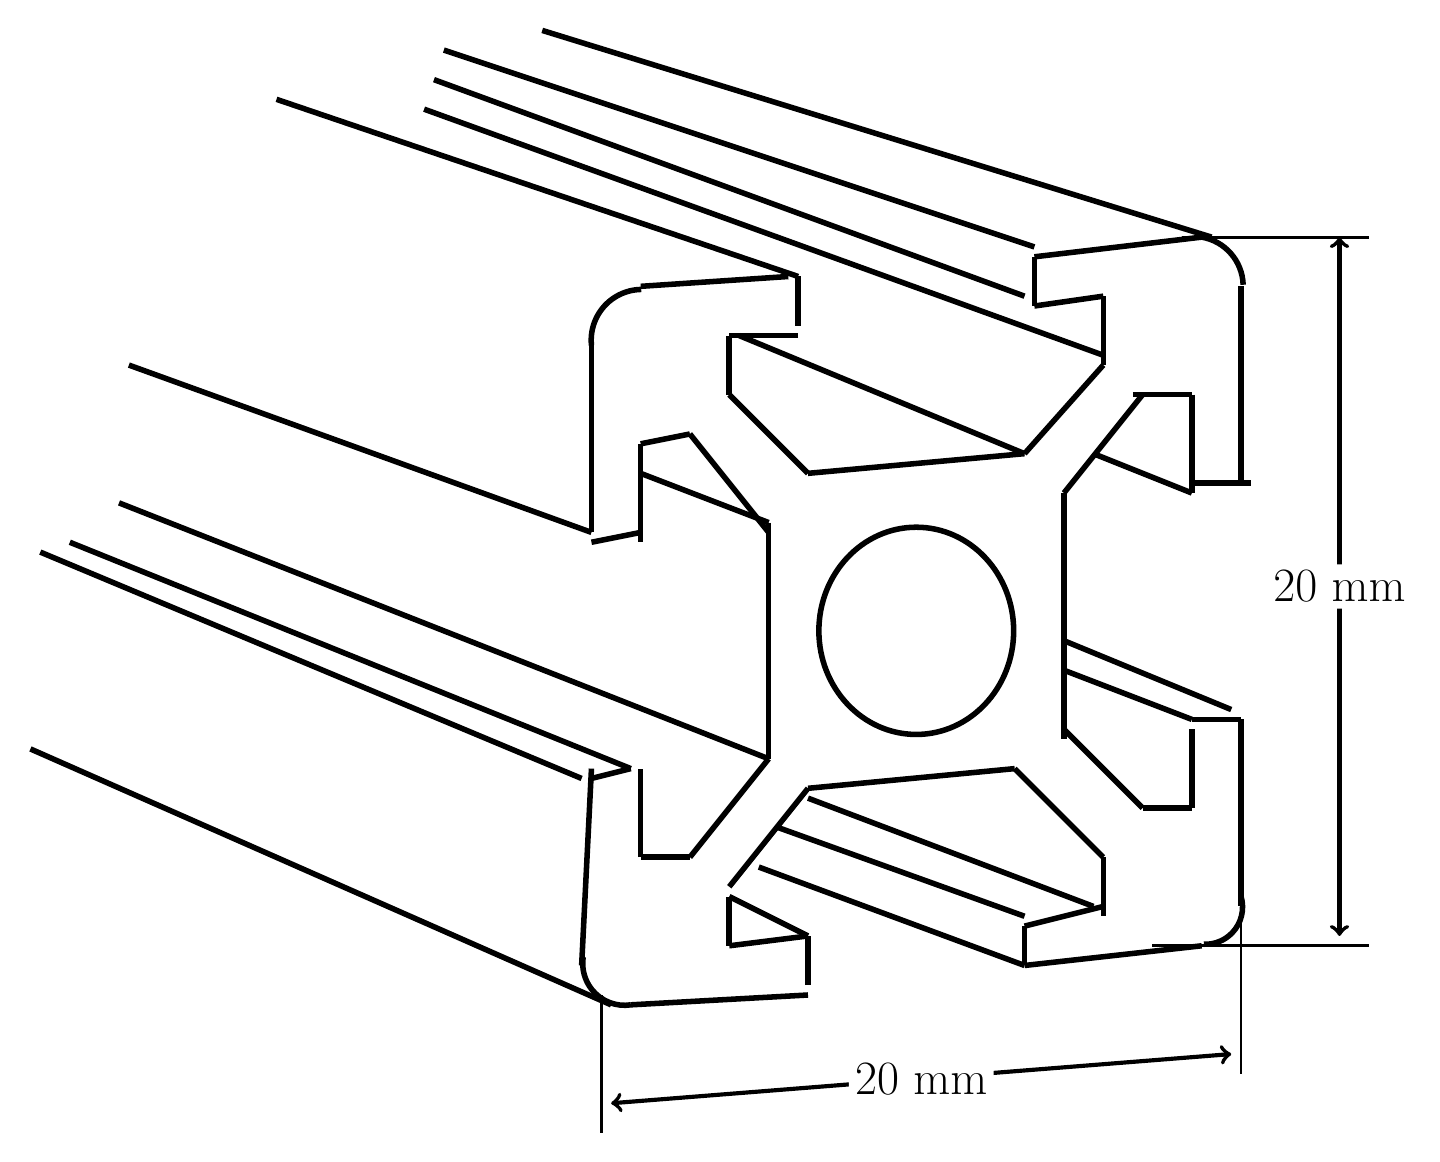
\begin{tikzpicture}
		\tikzstyle{every node}=[font=\fontsize{18.2pt}{23.7pt}\selectfont]
		
		\draw[line width=2pt] (1.875,14) -- (1.875,11.625);
		\draw[line width=2pt] (2.5,12.75) -- (2.5,11.5);
		\draw[line width=2pt] (2.5,14.75) -- (4.375,14.875);
		\draw[line width=2pt] (7.5,15.125) -- (9.625,15.375);
		\draw[line width=2pt] (10.125,14.75) -- (10.125,12.25);
		\draw[line width=2pt] (9.5,13.375) -- (9.5,12.125);
		\draw[line width=2pt] (8.875,13.375) -- (7.875,12.125);
		\draw[line width=2pt] (3.125,12.875) -- (4.125,11.625);
		\draw[line width=2pt] (4.125,11.75) -- (4.125,8.75);
		\draw[line width=2pt] (7.875,12.125) -- (7.875,9);
		\draw[line width=2pt] (4.125,8.75) -- (3.125,7.5);
		\draw[line width=2pt] (2.5,11.625) -- (1.875,11.5);
		\draw[line width=2pt] (3.125,7.5) -- (2.5,7.5);
		\draw[line width=2pt] (2.5,7.5) -- (2.5,8.625);
		\draw[line width=2pt] (2.375,8.625) -- (1.875,8.5);
		\draw[line width=2pt] (1.875,8.625) -- (1.75,6.125);
		\draw[line width=2pt] (2.375,5.625) -- (4.625,5.75);
		\draw[line width=2pt] (4.625,5.875) -- (4.625,6.5);
		\draw[line width=2pt] (4.625,6.5) -- (3.625,6.375);
		\draw[line width=2pt] (3.625,6.375) -- (3.625,7);
		\draw[line width=2pt] (3.625,7.125) -- (4.625,8.375);
		\draw[line width=2pt] (4.625,8.375) -- (7.25,8.625);
		\draw[line width=2pt] (7.25,8.625) -- (8.375,7.5);
		\draw[line width=2pt] (8.375,7.5) -- (8.375,6.75);
		\draw[line width=2pt] (8.375,6.875) -- (7.375,6.625);
		\draw[line width=2pt] (7.375,6.625) -- (7.375,6.125);
		\draw[line width=2pt] (7.375,6.125) -- (9.625,6.375);
		\draw[line width=2pt] (10.125,9.25) -- (10.125,6.875);
		\draw[line width=2pt] (10.125,9.25) -- (9.5,9.25);
		\draw[line width=2pt] (10,9.375) -- (7.875,10.25);
		\draw[line width=2pt] (9.5,9.25) -- (7.875,9.875);
		\draw[line width=2pt] (9.5,9.125) -- (9.5,8.125);
		\draw[line width=2pt] (9.5,8.125) -- (8.875,8.125);
		\draw[line width=2pt] (8.875,8.125) -- (7.875,9.125);
		\draw[line width=2pt] (3.625,13.375) -- (4.625,12.375);
		\draw[line width=2pt] (4.625,12.375) -- (7.375,12.625);
		\draw[line width=2pt] (7.375,12.625) -- (8.375,13.75);
		\draw[line width=2pt] (8.375,13.75) -- (8.375,14.625);
		\draw[line width=2pt] (8.375,14.625) -- (7.5,14.5);
		\draw[line width=2pt] (7.5,14.5) -- (7.5,15.125);
		\draw[line width=2pt] (4.5,14.875) -- (4.5,14.25);
		\draw[line width=2pt] (4.5,14.125) -- (3.625,14.125);
		\draw[line width=2pt] (3.625,14.125) -- (3.625,13.375);
		\draw[line width=2pt] (7.5,15.25) -- (0,17.75);
		\draw[line width=2pt] (4.5,14.875) -- (-2.125,17.125);
		\draw[line width=2pt] (7.375,14.625) -- (-0.125,17.375);
		\draw[line width=2pt] (7.375,12.625) -- (3.75,14.125);
		\draw[line width=2pt] (8.375,13.875) -- (-0.25,17);
		\draw[line width=2pt] (1.875,11.625) -- (-4,13.75);
		\draw[line width=2pt] (2.375,8.625) -- (-4.75,11.5);
		\draw[line width=2pt] (1.75,8.5) -- (-5.125,11.375);
		\draw[line width=2pt] (7.375,6.125) -- (4,7.375);
		\draw[line width=2pt] (7.375,6.75) -- (4.25,7.875);
		\draw[line width=2pt] (8.25,6.875) -- (4.625,8.25);
		\draw[line width=2pt] (4.125,8.75) -- (-4.125,12);
		
		\draw[line width=2pt, rotate around={-90:(6,10.375)}] (6,10.375) ellipse (1.3159317792358387cm and 1.2369758724816904cm);
		
		\draw[line width=2pt] (1.875,14) arc[start angle=-174.11, end angle=-269.15, radius=0.6446];
		\draw[line width=2pt] (9.625,15.375) arc[start angle=80.30, end angle=1.71, radius=0.6333];
		\draw[line width=2pt] (2.375,5.625) arc[start angle=-81.47, end angle=-188.53, radius=0.5323];
		\draw[line width=2pt] (10.125,7) arc[start angle=16.25, end angle=-92.34, radius=0.4733];
		
		\draw[line width=2pt] (2.5,12.75) -- (3.125,12.875);
		\draw[line width=2pt] (9.75,15.375) -- (1.25,18);
		\draw[line width=2pt] (2.125,5.625) -- (-5.25,8.875);
		\draw[line width=2pt] (4.625,6.5) -- (3.625,7);
		\draw[line width=2pt] (8.75,13.375) -- (9.5,13.375);
		\draw[line width=2pt] (9.5,12.125) -- (8.25,12.625);
		\draw[line width=2pt] (4.125,11.75) -- (2.5,12.375);
		\draw[line width=2pt] (9.5,12.25) -- (10.25,12.25);
		
		\draw[line width=1pt] (9.375,15.375) -- (11.75,15.375);
		\draw[line width=1pt] (9,6.375) -- (11.75,6.375);
		\draw[line width=1pt] (10.125,6.875) -- (10.125,4.75);
		\draw[line width=1pt] (2,5.75) -- (2,4);
		
		\draw[line width=1.5pt, <->] (2.125,4.375) -- (10,5)
		node[pos=0.5, fill=white, fill opacity=1, text opacity=1, inner xsep=0.080cm, inner ysep=0.085cm, rounded corners=0.020cm]{20 mm};
		
		\draw[line width=1.5pt, <->] (11.375,15.375) -- (11.375,6.5)
		node[pos=0.5, fill=white, fill opacity=1, text opacity=1, inner xsep=0.080cm, inner ysep=0.085cm, rounded corners=0.020cm]{20 mm};
		
	\end{tikzpicture}
}%


\textbf{Anzahl:} 6 Stück

\subsubsection{Creality Aluminium-Extrusionsprofil 40 x 20 mm}

Das Aluminiumprofil wird für stabilere Bereiche des Rahmens verwendet. Durch den größeren Querschnitt erhöht es die Steifigkeit der Konstruktion.

\textbf{Spezifikation:}
Maße: 40 x 20 x 509 mm
Material: Aluminium

\textbf{Anzahl:} 4 Stück

\subsubsection{Creality Aluminium-Extrusionsprofil 40 x 20 mm, ausgeklinkt}

Das ausgeklinkte Aluminiumprofil wird an angepassten Stellen des Rahmens eingesetzt. Die Ausklinkung ermöglicht die Montage in Bereichen mit begrenztem Bauraum.

\textbf{Spezifikation:}
Maße: 40 x 20 x 553 mm
Material: Aluminium
Besonderheit: ausgeklinkt

\textbf{Anzahl:} 2 Stück

\subsubsection{Creality Blech 4 mm für Riemenrolle}

Das Blech dient als Halterung für die Riemenrolle. Es fixiert die Rolle und unterstützt die Kraftübertragung des Riemenantriebs.

\resizebox{0.5\textwidth}{!}{%
	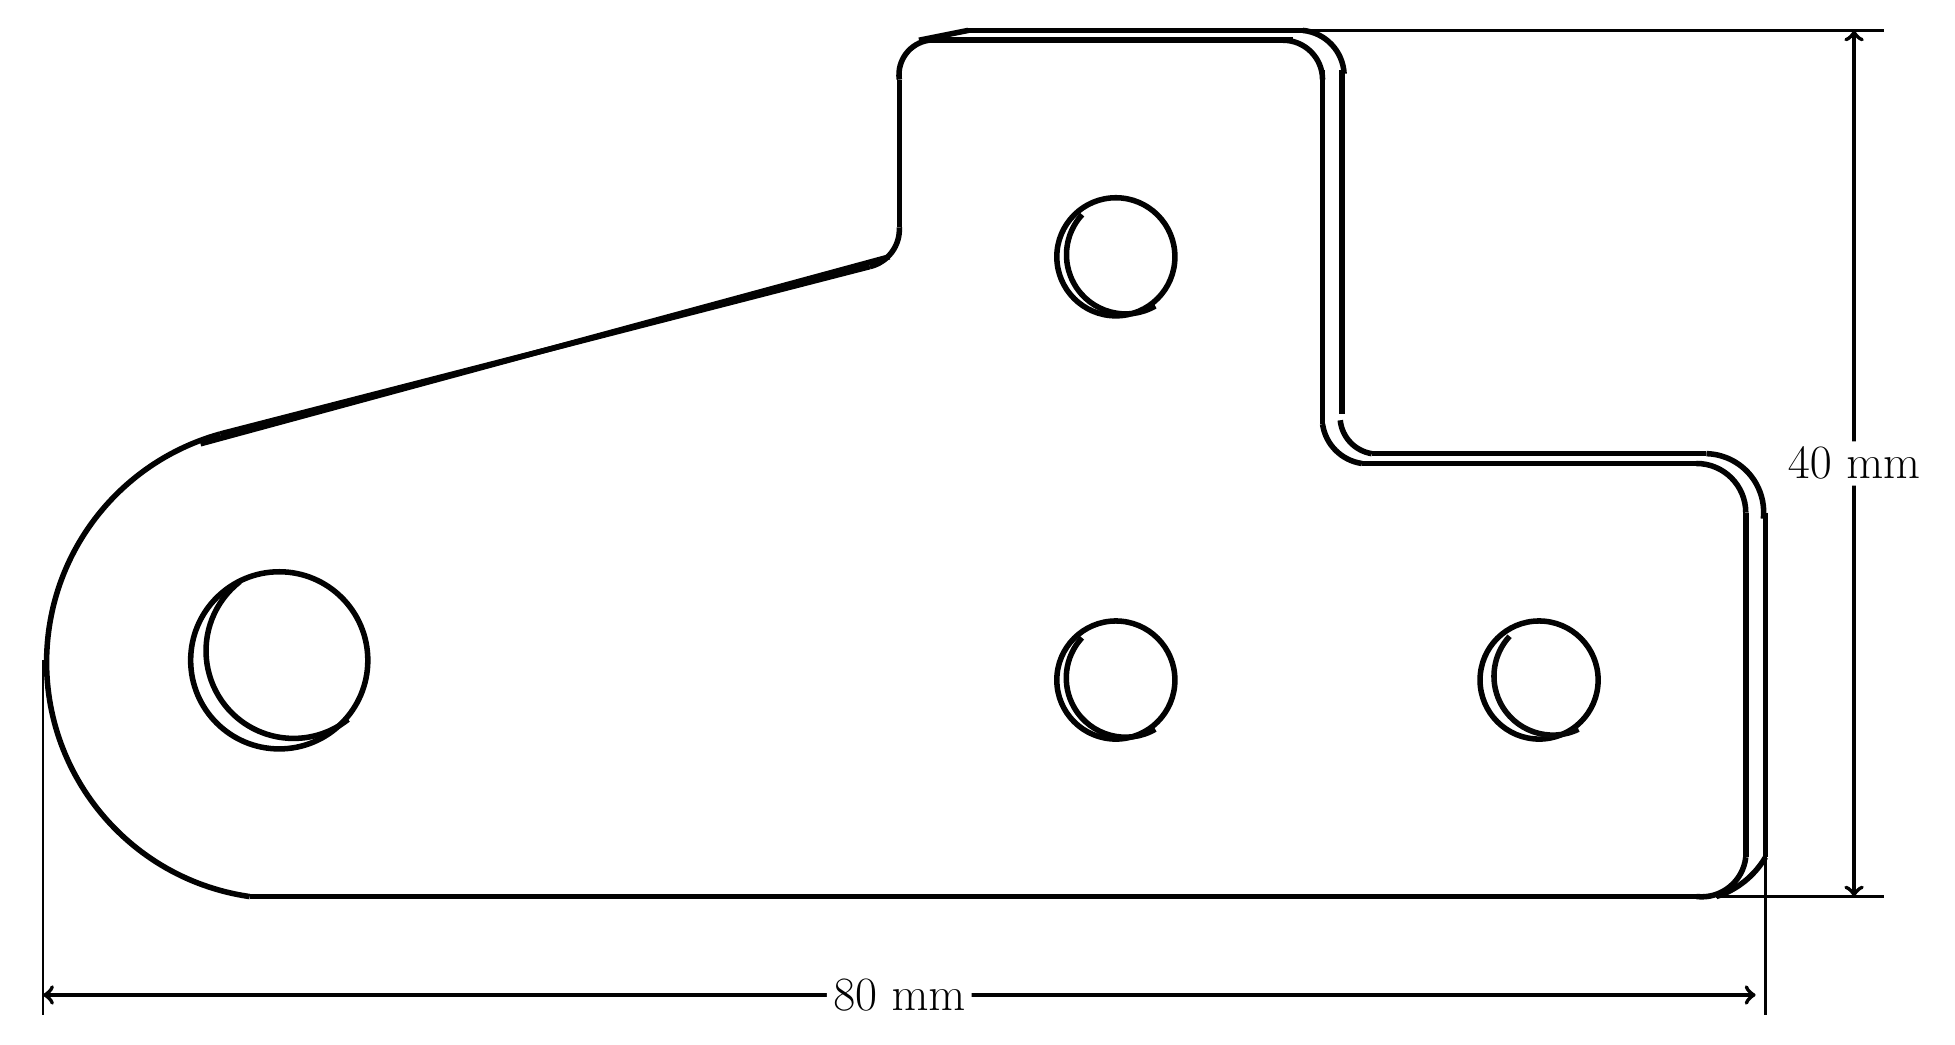
\begin{tikzpicture}
		\tikzstyle{every node}=[font=\fontsize{18.2pt}{23.7pt}\selectfont]
		
		\draw[color={rgb,255:red,2; green,2; blue,2}, draw opacity=1, line width=2pt] (-12.375,23.625) -- (-4.125,25.75);
		\draw[color={rgb,255:red,2; green,2; blue,2}, draw opacity=1, line width=2pt] (-3.75,28.125) -- (-3.75,26.25);
		\draw[color={rgb,255:red,2; green,2; blue,2}, draw opacity=1, line width=2pt] (-3.375,28.625) -- (1.25,28.625);
		\draw[color={rgb,255:red,2; green,2; blue,2}, draw opacity=1, line width=2pt] (1.625,28.25) -- (1.625,23.75);
		\draw[color={rgb,255:red,2; green,2; blue,2}, draw opacity=1, line width=2pt] (2.125,23.25) -- (6.375,23.25);
		\draw[color={rgb,255:red,2; green,2; blue,2}, draw opacity=1, line width=2pt] (7,22.625) -- (7,18.25);
		\draw[color={rgb,255:red,2; green,2; blue,2}, draw opacity=1, line width=2pt] (6.375,17.75) -- (-12,17.75);
		\draw[color={rgb,255:red,2; green,2; blue,2}, draw opacity=1, line width=2pt] (-12,17.75) arc[start angle=-98.18, end angle=-254.52, radius=3.0073];
		\draw[color={rgb,255:red,2; green,2; blue,2}, draw opacity=1, line width=2pt] (-3.75,26.25) arc[start angle=3.10, end angle=-76.84, radius=0.4865];
		\draw[color={rgb,255:red,2; green,2; blue,2}, draw opacity=1, line width=2pt] (-3.75,28.125) arc[start angle=-171.87, end angle=-261.87, radius=0.4419];
		\draw[color={rgb,255:red,2; green,2; blue,2}, draw opacity=1, line width=2pt] (1.125,28.625) arc[start angle=90.00, end angle=0.00, radius=0.5000];
		\draw[color={rgb,255:red,2; green,2; blue,2}, draw opacity=1, line width=2pt] (2.125,23.25) arc[start angle=-98.08, end angle=-171.92, radius=0.5886];
		\draw[color={rgb,255:red,2; green,2; blue,2}, draw opacity=1, line width=2pt] (6.375,23.25) arc[start angle=90.00, end angle=0.00, radius=0.6250];
		\draw[color={rgb,255:red,2; green,2; blue,2}, draw opacity=1, line width=2pt] (7,18.25) arc[start angle=-6.34, end angle=-96.34, radius=0.5660];
		
		\draw[color={rgb,255:red,2; green,2; blue,2}, draw opacity=1, line width=2pt] (-11.625,20.75) circle (1.125cm);
		\draw[color={rgb,255:red,2; green,2; blue,2}, draw opacity=1, line width=2pt] (-1,20.5) circle (0.75cm);
		\draw[color={rgb,255:red,2; green,2; blue,2}, draw opacity=1, line width=2pt] (-1,25.875) circle (0.75cm);
		\draw[color={rgb,255:red,2; green,2; blue,2}, draw opacity=1, line width=2pt] (4.375,20.5) circle (0.75cm);
		
		\draw[color={rgb,255:red,2; green,2; blue,2}, draw opacity=1, line width=2pt] (1.375,28.75) arc[start angle=84.39, end angle=2.75, radius=0.5812];
		\draw[color={rgb,255:red,2; green,2; blue,2}, draw opacity=1, line width=2pt] (1.375,28.75) -- (-2.875,28.75);
		\draw[color={rgb,255:red,2; green,2; blue,2}, draw opacity=1, line width=2pt] (-3.5,28.625) -- (-2.875,28.75);
		\draw[color={rgb,255:red,2; green,2; blue,2}, draw opacity=1, line width=2pt] (1.875,28.25) -- (1.875,23.875);
		\draw[color={rgb,255:red,2; green,2; blue,2}, draw opacity=1, line width=2pt] (2.25,23.375) -- (6.5,23.375);
		\draw[color={rgb,255:red,2; green,2; blue,2}, draw opacity=1, line width=2pt] (2.25,23.375) arc[start angle=-99.00, end angle=-174.30, radius=0.4774];
		\draw[color={rgb,255:red,2; green,2; blue,2}, draw opacity=1, line width=2pt] (7.25,22.625) -- (7.25,18.25);
		\draw[color={rgb,255:red,2; green,2; blue,2}, draw opacity=1, line width=2pt] (6.5,23.375) arc[start angle=88.54, end angle=-6.13, radius=0.7464];
		\draw[color={rgb,255:red,2; green,2; blue,2}, draw opacity=1, line width=2pt] (7.25,18.25) arc[start angle=-30.44, end angle=-72.24, radius=1.1220];
		\draw[color={rgb,255:red,2; green,2; blue,2}, draw opacity=1, line width=2pt] (-12.625,23.5) -- (-3.875,25.875);
		\draw[color={rgb,255:red,2; green,2; blue,2}, draw opacity=1, line width=2pt] (-10.75,20) arc[start angle=-51.53, end angle=-232.16, radius=1.1128];
		\draw[color={rgb,255:red,2; green,2; blue,2}, draw opacity=1, line width=2pt] (-0.5,25.25) arc[start angle=-60.03, end angle=-222.66, radius=0.7517];
		\draw[color={rgb,255:red,2; green,2; blue,2}, draw opacity=1, line width=2pt] (-0.5,19.875) arc[start angle=-59.95, end angle=-222.67, radius=0.7529];
		\draw[color={rgb,255:red,8; green,8; blue,8}, draw opacity=1, line width=2pt] (4.875,19.875) arc[start angle=-64.22, end angle=-222.69, radius=0.7479];
		
		\draw[color={rgb,255:red,2; green,2; blue,2}, draw opacity=1, line width=1pt] (-14.625,20.75) -- (-14.625,16.25);
		\draw[color={rgb,255:red,2; green,2; blue,2}, draw opacity=1, line width=1pt] (7.25,21) -- (7.25,16.25);
		\draw[color={rgb,255:red,2; green,2; blue,2}, draw opacity=1, line width=1pt] (1.375,28.75) -- (8.75,28.75);
		\draw[color={rgb,255:red,2; green,2; blue,2}, draw opacity=1, line width=1pt] (6.625,17.75) -- (8.75,17.75);
		
		\draw[color={rgb,255:red,2; green,2; blue,2}, draw opacity=1, line width=1.5pt, <->] 
		(8.375,28.75) -- (8.375,17.75)
		node[pos=0.5, fill={rgb,255:red,255; green,255; blue,255}, fill opacity=1, text opacity=1, inner xsep=0.080cm, inner ysep=0.085cm, rounded corners=0.020cm]{40 mm};
		
		\draw[color={rgb,255:red,2; green,2; blue,2}, draw opacity=1, line width=1.5pt, <->] 
		(-14.625,16.5) -- (7.125,16.5)
		node[pos=0.5, fill={rgb,255:red,255; green,255; blue,255}, fill opacity=1, text opacity=1, inner xsep=0.080cm, inner ysep=0.085cm, rounded corners=0.020cm]{80 mm};
		
	\end{tikzpicture}
}%

\textbf{Anzahl:} 2 Stück
\textbf{Spezifikation:}
Maße: 40 x 80 mm
Materialstärke: 4 mm
Material: Stahl

\subsubsection{Creality Eckwinkel}

Die Eckwinkel verbinden die Aluminiumprofile rechtwinklig miteinander. Dadurch wird der Rahmen stabilisiert.

\resizebox{0.5\textwidth}{!}{%
	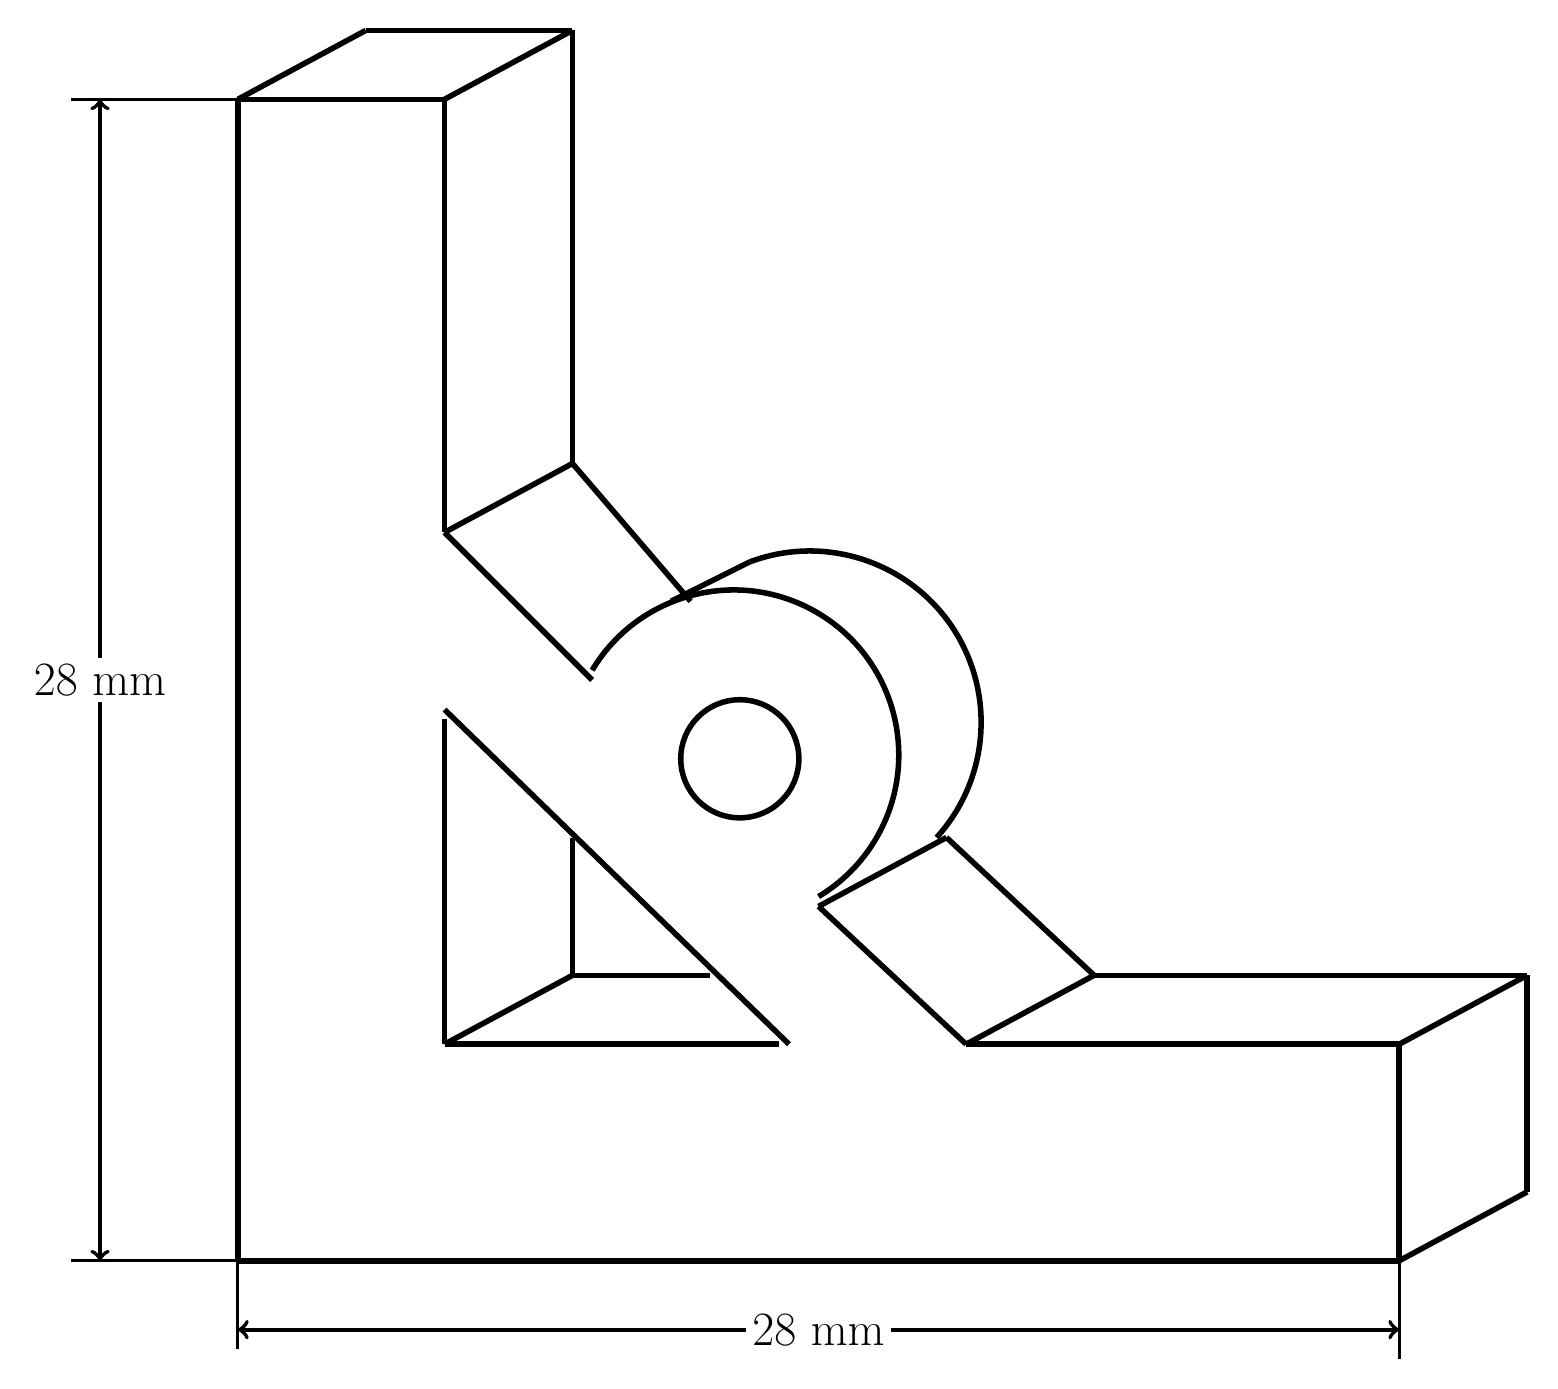
\begin{tikzpicture}
		\tikzstyle{every node}=[font=\fontsize{18.2pt}{23.7pt}\selectfont]
		
		\draw[line width=2pt] (-12.875,21.125) -- (-12.875,6.375);
		\draw[line width=2pt] (-12.875,21.125) -- (-10.25,21.125);
		\draw[line width=2pt] (-10.25,21.125) -- (-10.25,15.625);
		\draw[line width=2pt] (-10.25,15.625) -- (-8.375,13.75);
		\draw[line width=2pt] (-10.25,13.375) -- (-5.875,9.125);
		\draw[line width=2pt] (-10.25,13.25) -- (-10.25,9.125);
		\draw[line width=2pt] (-10.25,9.125) -- (-6,9.125);
		\draw[line width=2pt] (-12.875,6.375) -- (1.875,6.375);
		\draw[line width=2pt] (1.875,9.125) -- (1.875,6.375);
		\draw[line width=2pt] (-5.5,10.875) -- (-3.625,9.125);
		\draw[line width=2pt] (-3.625,9.125) -- (1.875,9.125);
		\draw[line width=2pt] (-12.875,21.125) -- (-11.25,22);
		\draw[line width=2pt] (-10.25,21.125) -- (-8.625,22);
		\draw[line width=2pt] (-10.25,15.625) -- (-8.625,16.5);
		\draw[line width=2pt] (-5.5,10.875) -- (-3.875,11.75);
		\draw[line width=2pt] (-10.25,9.125) -- (-8.625,10);
		\draw[line width=2pt] (1.875,9.125) -- (3.5,10);
		\draw[line width=2pt] (1.875,6.375) -- (3.5,7.25);
		\draw[line width=2pt] (-11.25,22) -- (-8.625,22);
		\draw[line width=2pt] (-2,10) -- (3.5,10);
		\draw[line width=2pt] (-3.625,9.125) -- (-2,10);
		\draw[line width=2pt] (-8.625,22) -- (-8.625,16.5);
		\draw[line width=2pt] (-8.625,16.5) -- (-7.125,14.75);
		\draw[line width=2pt] (-3.875,11.75) -- (-2,10);
		\draw[line width=2pt] (-8.625,10) -- (-6.875,10);
		\draw[line width=2pt] (-8.625,10) -- (-8.625,11.75);
		\draw[line width=2pt] (-8.375,13.875) arc[start angle=149.08, end angle=-59.08, radius=2.0959];
		\draw[line width=2pt] (-6.375,15.25) arc (110.56:-42.24:2.1759);
		\draw[line width=2pt] (-7.375,14.75) -- (-6.375,15.25);
		\draw[line width=2pt] (3.5,10) -- (3.5,7.25);
		\draw[line width=2pt] (-6.5,12.75) circle (0.75cm);
		
		\draw[line width=1pt] (-12.875,21.125) -- (-15,21.125);
		\draw[line width=1pt] (-12.875,6.375) -- (-15,6.375);
		\draw[line width=1pt] (-12.875,6.375) -- (-12.875,5.25);
		\draw[line width=1pt] (1.875,6.375) -- (1.875,5.125);
		
		\draw[line width=1.5pt, <->] (-14.625,21.125) -- (-14.625,6.375)
		node[pos=0.5, fill=white, fill opacity=1, text opacity=1, inner xsep=0.080cm, inner ysep=0.085cm, rounded corners=0.020cm]{28 mm};
		
		\draw[line width=1.5pt, <->] (-12.875,5.5) -- (1.875,5.5)
		node[pos=0.5, fill=white, fill opacity=1, text opacity=1, inner xsep=0.080cm, inner ysep=0.085cm, rounded corners=0.020cm]{28 mm};
		
	\end{tikzpicture}
}%
\textbf{Spezifikation:}
Maße: 28 x 28 mm
Materialstärke: 4 mm
Material: Aluminium
\textbf{Anzahl:} 4 Stück



\subsubsection{Druckteil Eckhalter 1}

Der Eckhalter dient als zusätzliches Verbindungselement am Grundrahmen. Er unterstützt die Befestigung einzelner Rahmenteile.

\resizebox{0.5\textwidth}{!}{%
	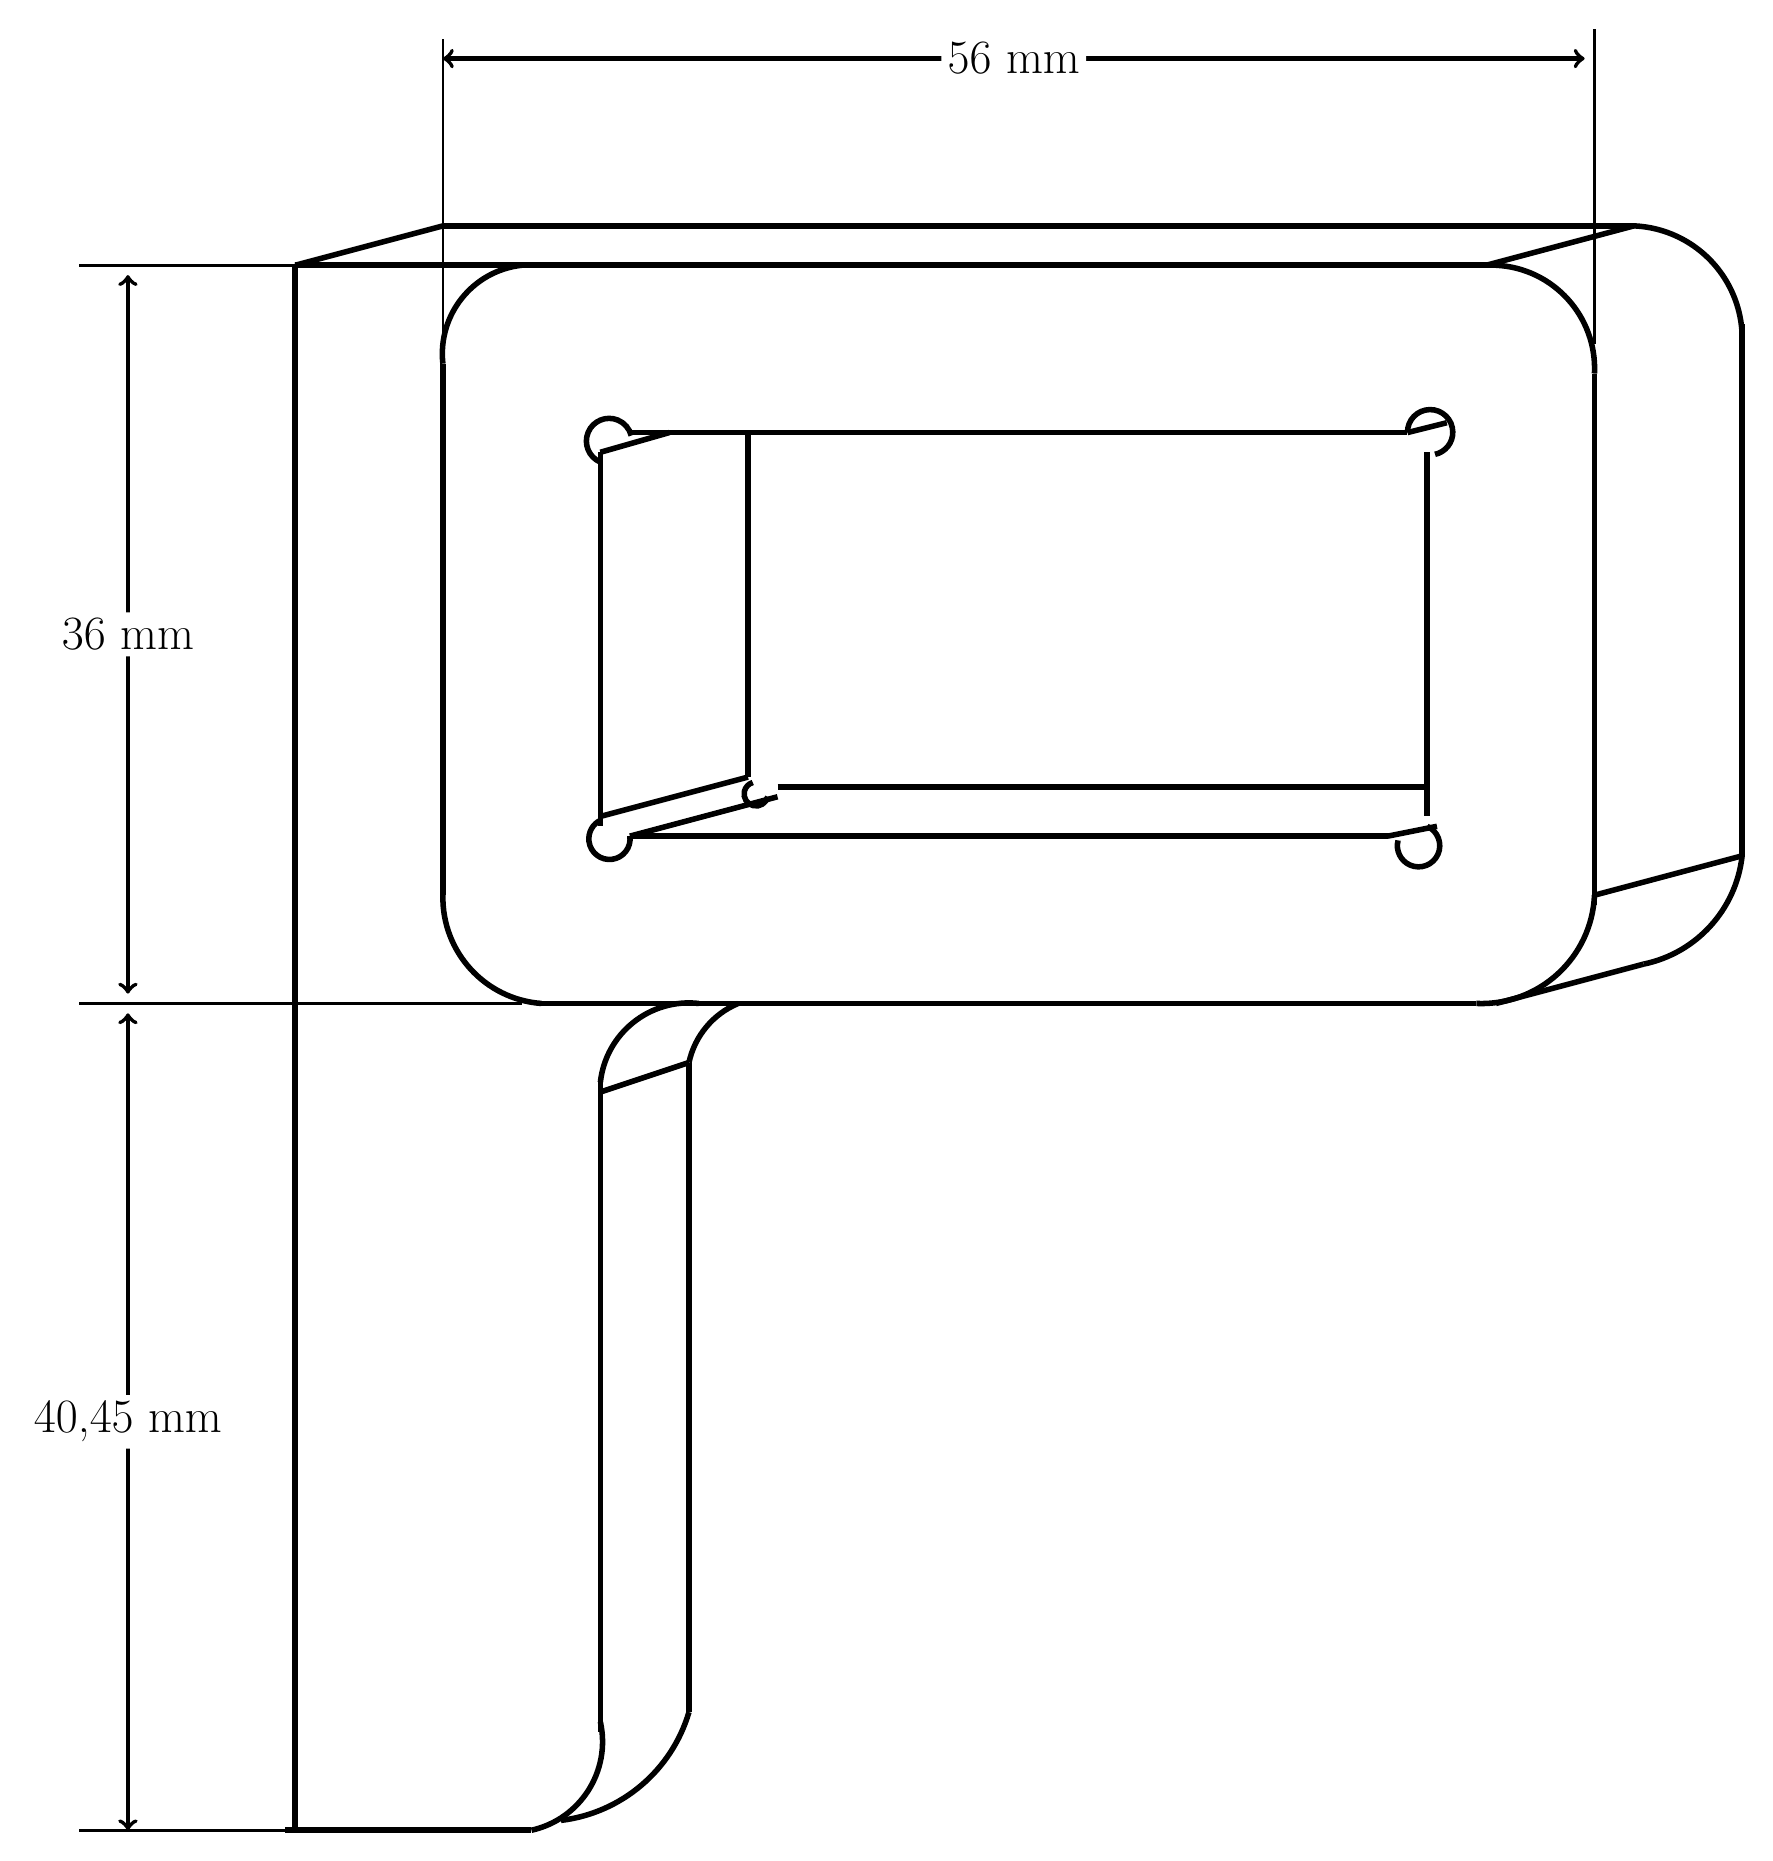
\begin{tikzpicture}
		\tikzstyle{every node}=[font=\fontsize{18.2pt}{23.7pt}\selectfont]
		
		\draw[line width=2pt] (-9.625,20.375) -- (-9.625,0.5);
		\draw[line width=2pt] (-9.625,20.375) -- (5.625,20.375);
		\draw[line width=2pt] (-9.75,0.5) -- (-6.625,0.5);
		\draw[line width=2pt] (-5.75,10) -- (-5.75,1.75);
		\draw[line width=2pt] (-6.5,11) -- (5.375,11);
		\draw[line width=2pt] (6.875,19) -- (6.875,12.25);
		\draw[line width=2pt] (-5.375,13.125) -- (4.25,13.125);
		\draw[line width=2pt] (4.75,18) -- (4.75,13.375);
		\draw[line width=2pt] (-5.75,18) -- (-5.75,13.25);
		\draw[line width=2pt] (-7.75,19.125) -- (-7.75,12.375);
		\draw[line width=2pt] (-7.75,19.125) arc[start angle=-173.66, end angle=-263.66, radius=1.1319];
		\draw[line width=2pt] (5.625,20.375) arc[start angle=87.27, end angle=-2.73, radius=1.3140];
		\draw[line width=2pt] (6.875,12.375) arc[start angle=-2.49, end angle=-92.49, radius=1.4389];
		\draw[line width=2pt] (-5.75,10) arc[start angle=173.66, end angle=83.66, radius=1.1319];
		\draw[line width=2pt] (-6.5,11) arc[start angle=-94.21, end angle=-181.25, radius=1.3493];
		\draw[line width=2pt] (-5.75,1.875) arc[start angle=12.53, end angle=-77.47, radius=1.1524];
		\draw[line width=2pt] (-9.625,20.375) -- (-7.75,20.875);
		\draw[line width=2pt] (-5.75,13.375) -- (-3.875,13.875);
		\draw[line width=2pt] (-5.375,13.125) -- (-3.5,13.625);
		\draw[line width=2pt] (4.25,13.125) -- (4.875,13.25);
		\draw[line width=2pt] (-5.375,13.125) arc[start angle=7.54, end angle=-245.16, radius=0.2620];
		\draw[line width=2pt] (-5.75,17.875) arc[start angle=-112.67, end angle=-346.01, radius=0.2890];
		\draw[line width=2pt] (4.5,18.25) arc[start angle=-179.14, end angle=-437.47, radius=0.2878];
		\draw[line width=2pt] (-5.375,18.25) -- (4.5,18.25);
		\draw[line width=2pt] (4.75,13.25) arc[start angle=66.09, end angle=-194.42, radius=0.2692];
		\draw[line width=2pt] (-3.625,13.625) arc[start angle=-13.27, end angle=-253.97, radius=0.1519];
		\draw[line width=2pt] (-3.875,13.875) -- (-3.875,18.25);
		\draw[line width=2pt] (-3.5,13.75) -- (4.75,13.75);
		\draw[line width=2pt] (4.5,18.25) -- (5,18.375);
		\draw[line width=2pt] (-7.75,20.875) -- (7.375,20.875);
		\draw[line width=2pt] (5.5,20.375) -- (7.375,20.875);
		\draw[line width=2pt] (7.25,20.875) arc[start angle=92.60, end angle=2.38, radius=1.4361];
		\draw[line width=2pt] (8.75,19.625) -- (8.75,12.875);
		\draw[line width=2pt] (8.75,12.875) arc[start angle=-6.30, end angle=-78.24, radius=1.5819];
		\draw[line width=2pt] (5.625,11) -- (7.5,11.5);
		\draw[line width=2pt] (6.875,12.375) -- (8.75,12.875);
		\draw[line width=2pt] (-5.75,9.875) -- (-4.625,10.25);
		\draw[line width=2pt] (-4.625,10.25) arc[start angle=167.81, end angle=112.57, radius=1.0529];
		\draw[line width=2pt] (-4.625,10.25) -- (-4.625,2);
		\draw[line width=2pt] (-4.625,2) arc[start angle=-16.44, end angle=-83.09, radius=1.9374];
		
		\draw[line width=1pt] (-9.625,20.375) -- (-12.375,20.375);
		\draw[line width=1pt] (-9.625,0.5) -- (-12.375,0.5);
		\draw[line width=1pt] (-7.75,19.5) -- (-7.75,23.25);
		\draw[line width=1pt] (6.875,19.375) -- (6.875,23.375);
		
		\draw[line width=1.5pt, <->] (-7.75,23) -- (6.75,23)
		node[pos=0.5, fill=white, fill opacity=1, text opacity=1, inner xsep=0.080cm, inner ysep=0.085cm, rounded corners=0.020cm]{56 mm};
		
		\draw[line width=1.5pt, <->] (-11.75,20.25) -- (-11.75,11.125)
		node[pos=0.5, fill=white, fill opacity=1, text opacity=1, inner xsep=0.080cm, inner ysep=0.085cm, rounded corners=0.020cm]{36 mm};
		
		\draw[line width=1pt] (-6.75,11) -- (-12.375,11);
		
		\draw[line width=1.5pt, <->] (-11.75,10.875) -- (-11.75,0.5)
		node[pos=0.5, fill=white, fill opacity=1, text opacity=1, inner xsep=0.080cm, inner ysep=0.085cm, rounded corners=0.020cm]{40,45 mm};
		
		\draw[line width=2pt] (-5.75,18) -- (-4.875,18.25);
		
	\end{tikzpicture}
}%
\textbf{Spezifikation:}
Maße: 28 x 28 mm
Materialstärke: 4 mm
Material: Aluminium
\textbf{Anzahl:} 1 Stück

\subsubsection{Druckteil Eckhalter 2}

Der Eckhalter dient als weiteres Verbindungselement am Grundrahmen. Er wird zur zusätzlichen Befestigung oder Ausrichtung verwendet.

\textbf{Spezifikation:}
Maße: 76,45 x 56 mm
Material: PETG

\textbf{Anzahl:} 1 Stück

\subsubsection{Creality Nutenstein}

Der Nutenstein wird in die Nut der Aluminiumprofile eingesetzt. Er dient als Gewindeelement zur Befestigung von Schrauben.

\resizebox{0.5\textwidth}{!}{%
	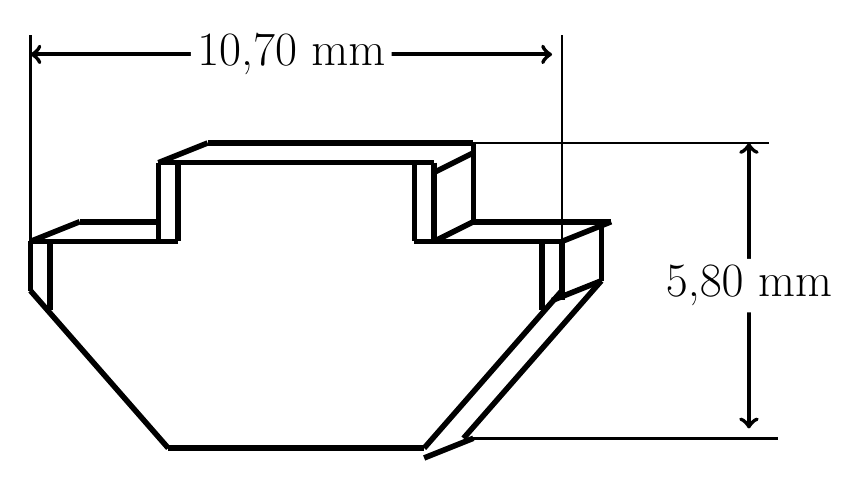
\begin{tikzpicture}
		\tikzstyle{every node}=[font=\fontsize{18.2pt}{23.7pt}\selectfont]
		
		\draw[line width=2pt] (-4.875,10.875) -- (-1.375,10.875);
		\draw[line width=2pt] (-4.875,10.875) -- (-4.875,9.875);
		\draw[line width=2pt] (-4.625,10.875) -- (-4.625,9.875);
		\draw[line width=2pt] (-4.625,9.875) -- (-6.5,9.875);
		\draw[line width=2pt] (-6.5,9.875) -- (-6.5,9.25);
		\draw[line width=2pt] (-6.25,9.875) -- (-6.25,9);
		\draw[line width=2pt] (-6.5,9.25) -- (-4.75,7.25);
		\draw[line width=2pt] (-4.75,7.25) -- (-1.5,7.25);
		\draw[line width=2pt] (-1.5,7.25) -- (0.25,9.25);
		\draw[line width=2pt] (0,9.875) -- (0,9);
		\draw[line width=2pt] (0.25,9.875) -- (0.25,9.125);
		\draw[line width=2pt] (-1.375,10.875) -- (-1.375,9.875);
		\draw[line width=2pt] (-1.625,10.875) -- (-1.625,9.875);
		\draw[line width=2pt] (-1.625,9.875) -- (0.25,9.875);
		\draw[line width=2pt] (-4.875,10.875) -- (-4.25,11.125);
		\draw[line width=2pt] (-4.25,11.125) -- (-0.875,11.125);
		\draw[line width=2pt] (-6.5,9.875) -- (-5.875,10.125);
		\draw[line width=2pt] (-1.375,9.875) -- (-0.875,10.125);
		\draw[line width=2pt] (0.25,9.875) -- (0.875,10.125);
		\draw[line width=2pt] (0.125,9.125) -- (0.75,9.375);
		\draw[line width=2pt] (-5.875,10.125) -- (-4.875,10.125);
		\draw[line width=2pt] (-1.375,10.75) -- (-0.875,11);
		\draw[line width=2pt] (-0.875,11.125) -- (-0.875,10.125);
		\draw[line width=2pt] (-0.875,10.125) -- (0.875,10.125);
		\draw[line width=2pt] (0.75,10.125) -- (0.75,9.375);
		\draw[line width=2pt] (-1,7.375) -- (0.75,9.375);
		\draw[line width=2pt] (-1.5,7.125) -- (-0.875,7.375);
		
		\draw[line width=1pt] (-6.5,9.625) -- (-6.5,12.5);
		\draw[line width=1pt] (0.25,9.625) -- (0.25,12.5);
		\draw[line width=1pt] (-0.875,11.125) -- (2.875,11.125);
		\draw[line width=1pt] (-0.875,7.375) -- (3,7.375);
		
		\draw[line width=1.5pt, <->] (2.625,11.125) -- (2.625,7.5)
		node[pos=0.5, fill=white, fill opacity=1, text opacity=1, inner xsep=0.080cm, inner ysep=0.085cm, rounded corners=0.020cm]{5,80 mm};
		
		\draw[line width=1.5pt, <->] (-6.5,12.25) -- (0.125,12.25)
		node[pos=0.5, fill=white, fill opacity=1, text opacity=1, inner xsep=0.080cm, inner ysep=0.085cm, rounded corners=0.020cm]{10,70 mm};
		
	\end{tikzpicture}
}%
\textbf{Spezifikation:}
Material: PETG
\textbf{Anzahl:} 8 Stück

\subsubsection{Druckteil Nutenstein-Block}

Der Nutenstein-Block dient als zusätzliches Befestigungselement an den Profilnuten. Er ermöglicht die Montage weiterer Bauteile am Rahmen.

\textbf{Spezifikation:}
Material: PETG

\textbf{Anzahl:} 4 Stück

\subsubsection{Holzplatte}

Die Holzplatte dient als Montage- oder Auflagefläche innerhalb der Konstruktion. Sie kann zur Befestigung weiterer Bauteile genutzt werden.

\resizebox{0.5\textwidth}{!}{%
	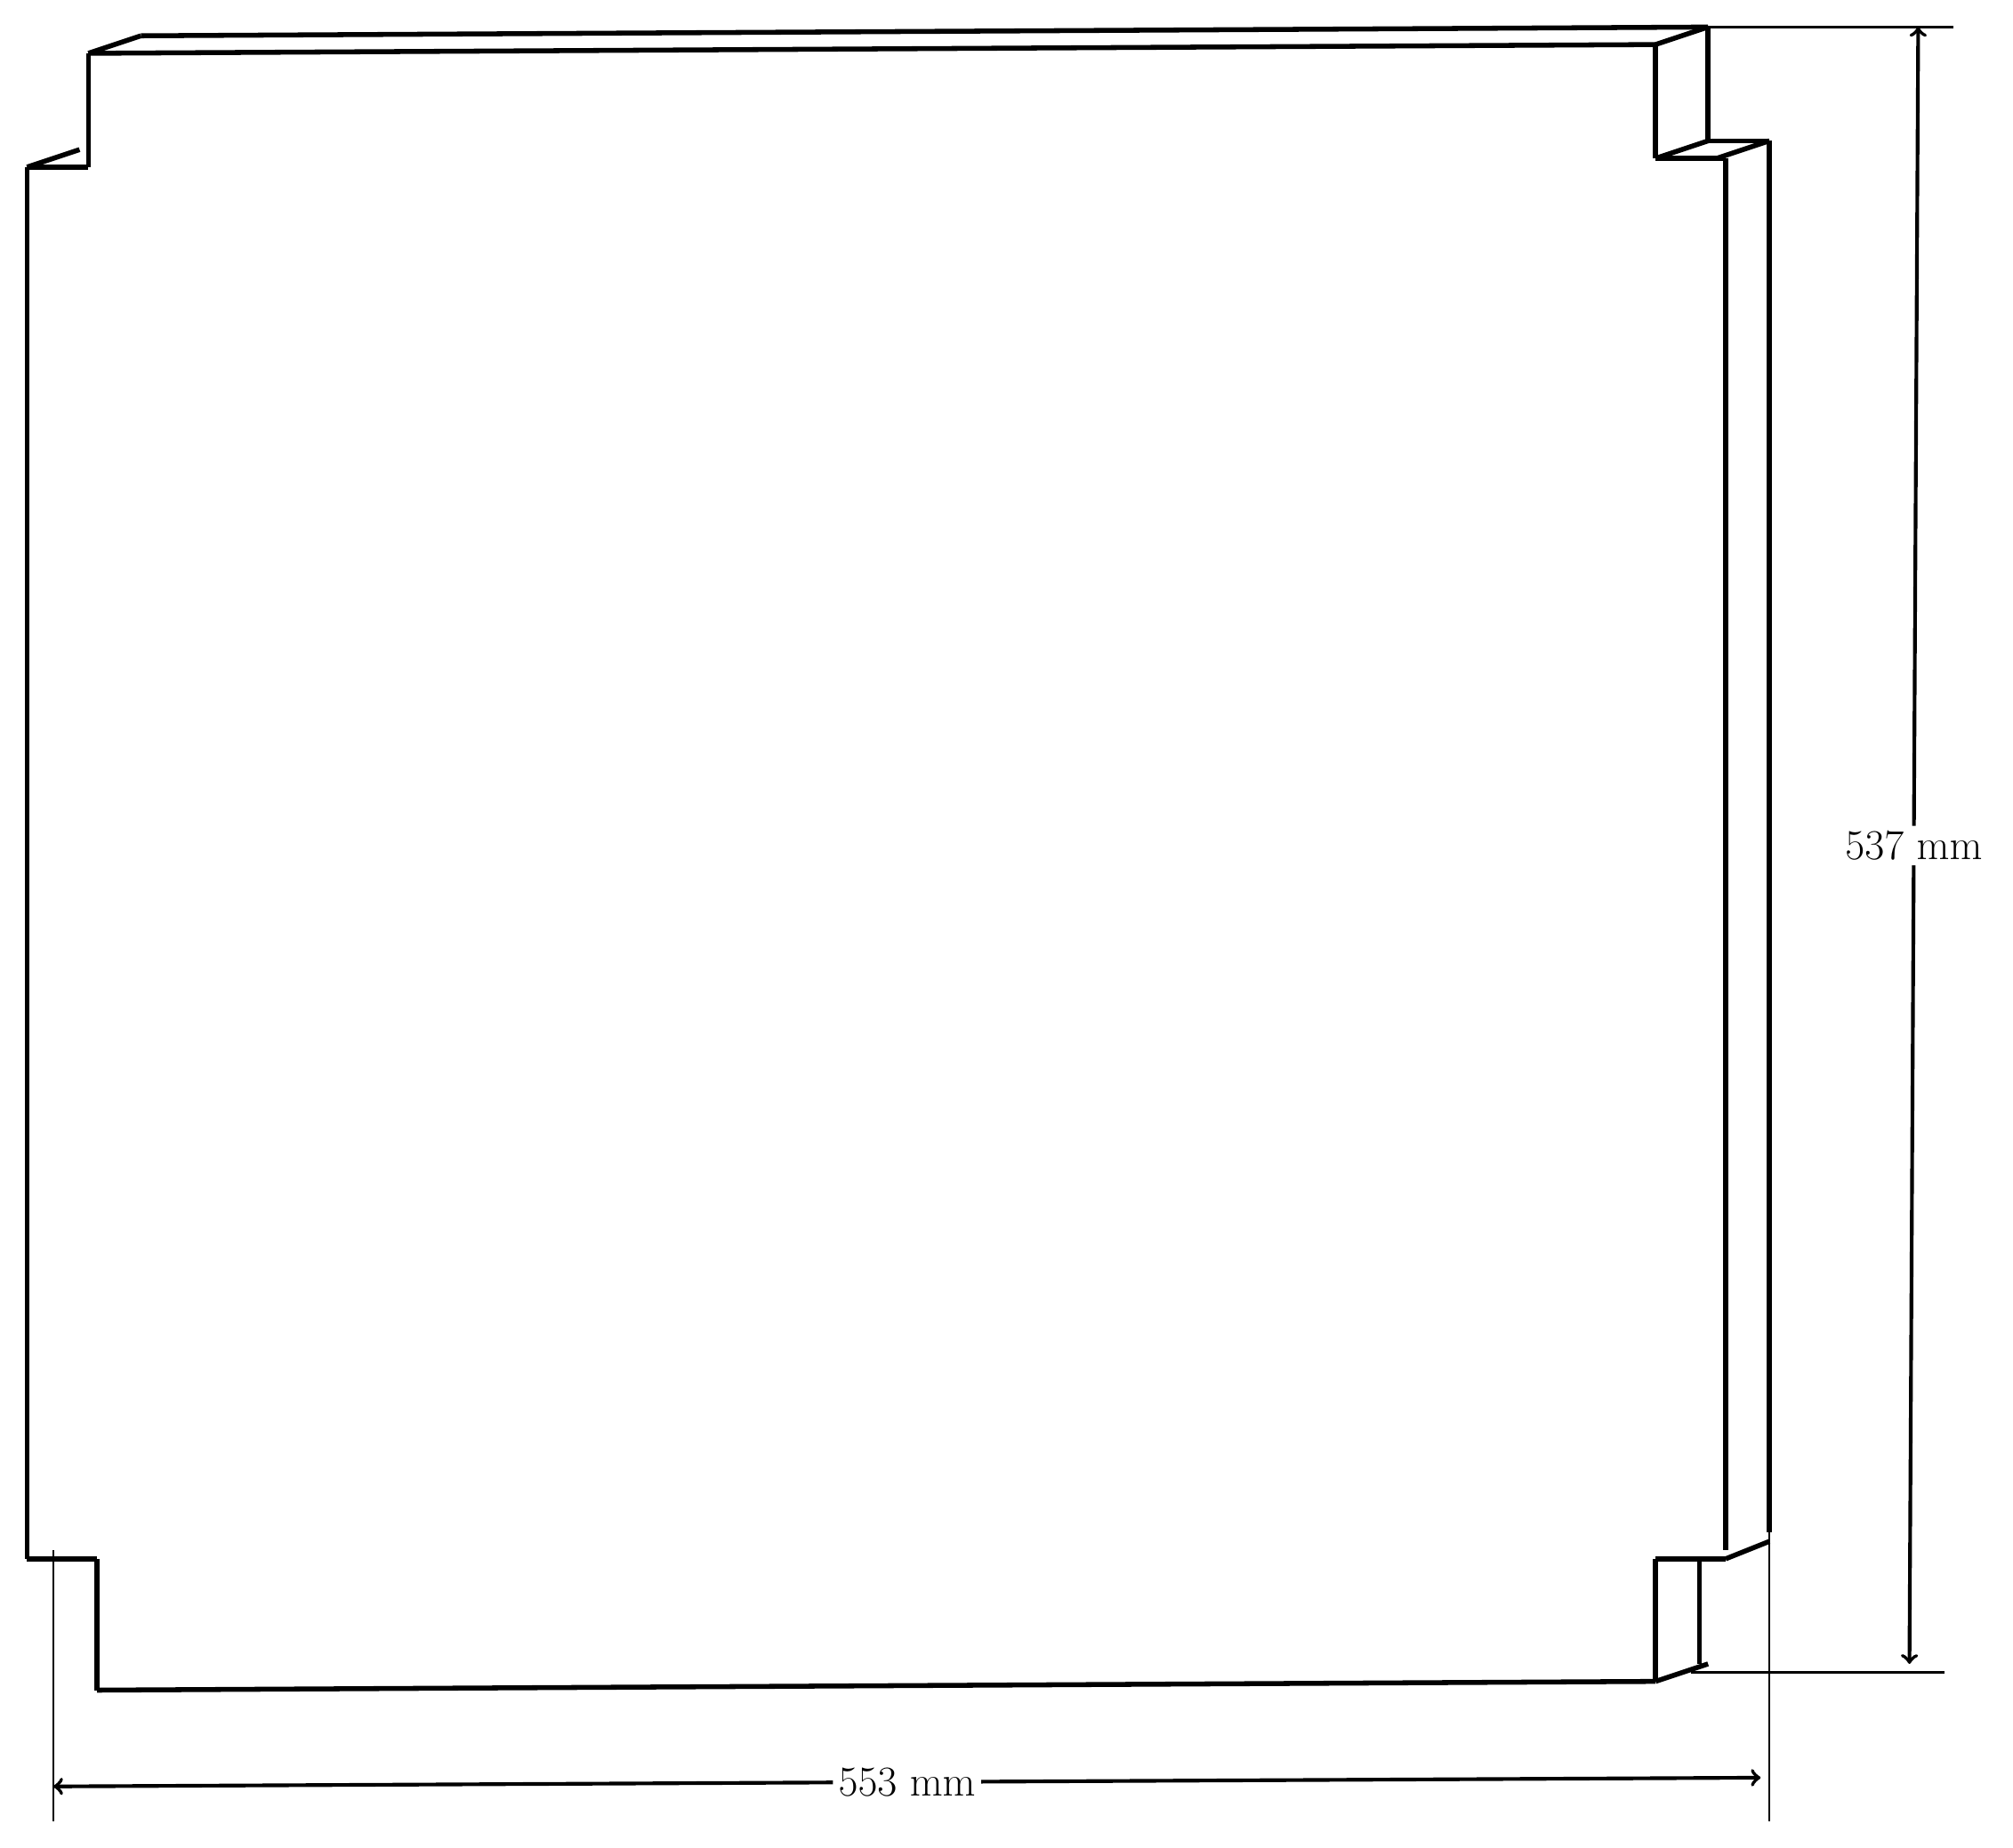
\begin{tikzpicture}
		\tikzstyle{every node}=[font=\fontsize{18.2pt}{23.7pt}\selectfont]
		
		\draw[line width=2pt] (-13,26.125) -- (-13,6.25);
		\draw[line width=2pt] (-13,26.125) -- (-12.125,26.125);
		\draw[line width=2pt] (-12.125,26.125) -- (-12.125,27.75);
		\draw[line width=2pt] (-12.125,27.75) -- (10.25,27.875);
		\draw[line width=2pt] (10.25,27.875) -- (10.25,26.25);
		\draw[line width=2pt] (10.25,26.25) -- (11.25,26.25);
		\draw[line width=2pt] (11.25,26.25) -- (11.25,6.375);
		\draw[line width=2pt] (11.25,6.25) -- (10.25,6.25);
		\draw[line width=2pt] (10.25,6.25) -- (10.25,4.5);
		\draw[line width=2pt] (10.25,4.5) -- (-12,4.375);
		\draw[line width=2pt] (-12,4.375) -- (-12,6.25);
		\draw[line width=2pt] (-13,6.25) -- (-12,6.25);
		\draw[line width=2pt] (-13,26.125) -- (-12.25,26.375);
		\draw[line width=2pt] (-12.125,27.75) -- (-11.375,28);
		\draw[line width=2pt] (10.25,27.875) -- (11,28.125);
		\draw[line width=2pt] (10.25,26.25) -- (11,26.5);
		\draw[line width=2pt] (11.125,26.25) -- (11.875,26.5);
		\draw[line width=2pt] (10.25,4.5) -- (11,4.75);
		\draw[line width=2pt] (-11.375,28) -- (11,28.125);
		\draw[line width=2pt] (11,28.125) -- (11,26.5);
		\draw[line width=2pt] (11,26.5) -- (11.875,26.5);
		\draw[line width=2pt] (11.875,26.5) -- (11.875,6.625);
		\draw[line width=2pt] (11.25,6.25) -- (11.875,6.5);
		\draw[line width=2pt] (10.875,6.25) -- (10.875,4.75);
		
		\draw[line width=1pt] (11,28.125) -- (14.5,28.125);
		\draw[line width=1pt] (10.75,4.625) -- (14.375,4.625);
		\draw[line width=1pt] (11.875,6.75) -- (11.875,2.5);
		\draw[line width=1pt] (-12.625,6.375) -- (-12.625,2.5);
		
		\draw[line width=1.5pt, <->] (14,28.125) -- (13.875,4.75)
		node[pos=0.5, fill=white, fill opacity=1, text opacity=1, inner xsep=0.080cm, inner ysep=0.085cm, rounded corners=0.020cm]{537 mm};
		
		\draw[line width=1.5pt, <->] (-12.625,3) -- (11.75,3.125)
		node[pos=0.5, fill=white, fill opacity=1, text opacity=1, inner xsep=0.080cm, inner ysep=0.085cm, rounded corners=0.020cm]{553 mm};
		
	\end{tikzpicture}
}%

\textbf{Anzahl:} 1 Stück
